\section{Results from test runs}
\label{sec:resul}
All the results shown below are derived by running FjordOs CL on the Vilje supercomputer at the Norwegian High Performance Computing facilities in Trondheim. We show results from a hindcast initialized from NorKyst800 on April 1st, 2014 and continued up to and including the month of December 2015. All inputs are as described in Section \ref{subsec:atmos}.
 
The results from the hindcast are further discussed and evaluated in some detail in an upcoming report \citep{hjelm:etal:2016}. Here we merely present snapshots of fields of currents, temperature, salinity and sea level on March 23, 2015, that is, about one year after commencing the simulation. To properly reveal and appreciate the level of details provided by the FjordOs CL model the simulated currents are shown for selected parts of the fjord (Section \ref{subsec:curre}). Regarding temperature (Section \ref{subsec:tempe}), salinity (Section \ref{subsec:salin}) and sea level (Section \ref{subsec:seale}) the whole computational domain covered by the FjordOs CL model is displayed. 

\subsection{Currents}
\label{subsec:curre}
Focussing first on currents in the inner Oslofjord (Figures \ref{fig:curr_oslo}) we note the detailed current pattern returned by the FjordOs CL model. Although the speed is low compared to other parts of the fjord, e.g. in the {\DR} Sound (Figure \ref{fig:curr_drobak}) the pattern is rich in detail. 
 %%%%%%%%%%%%%%%%%%% Figure  %%%%%%%%%%%%%%%
\begin{figure}[t]
  \begin{pspicture}(0,0)(15,12)
% Include graphs
	\rput[b](7.5,0){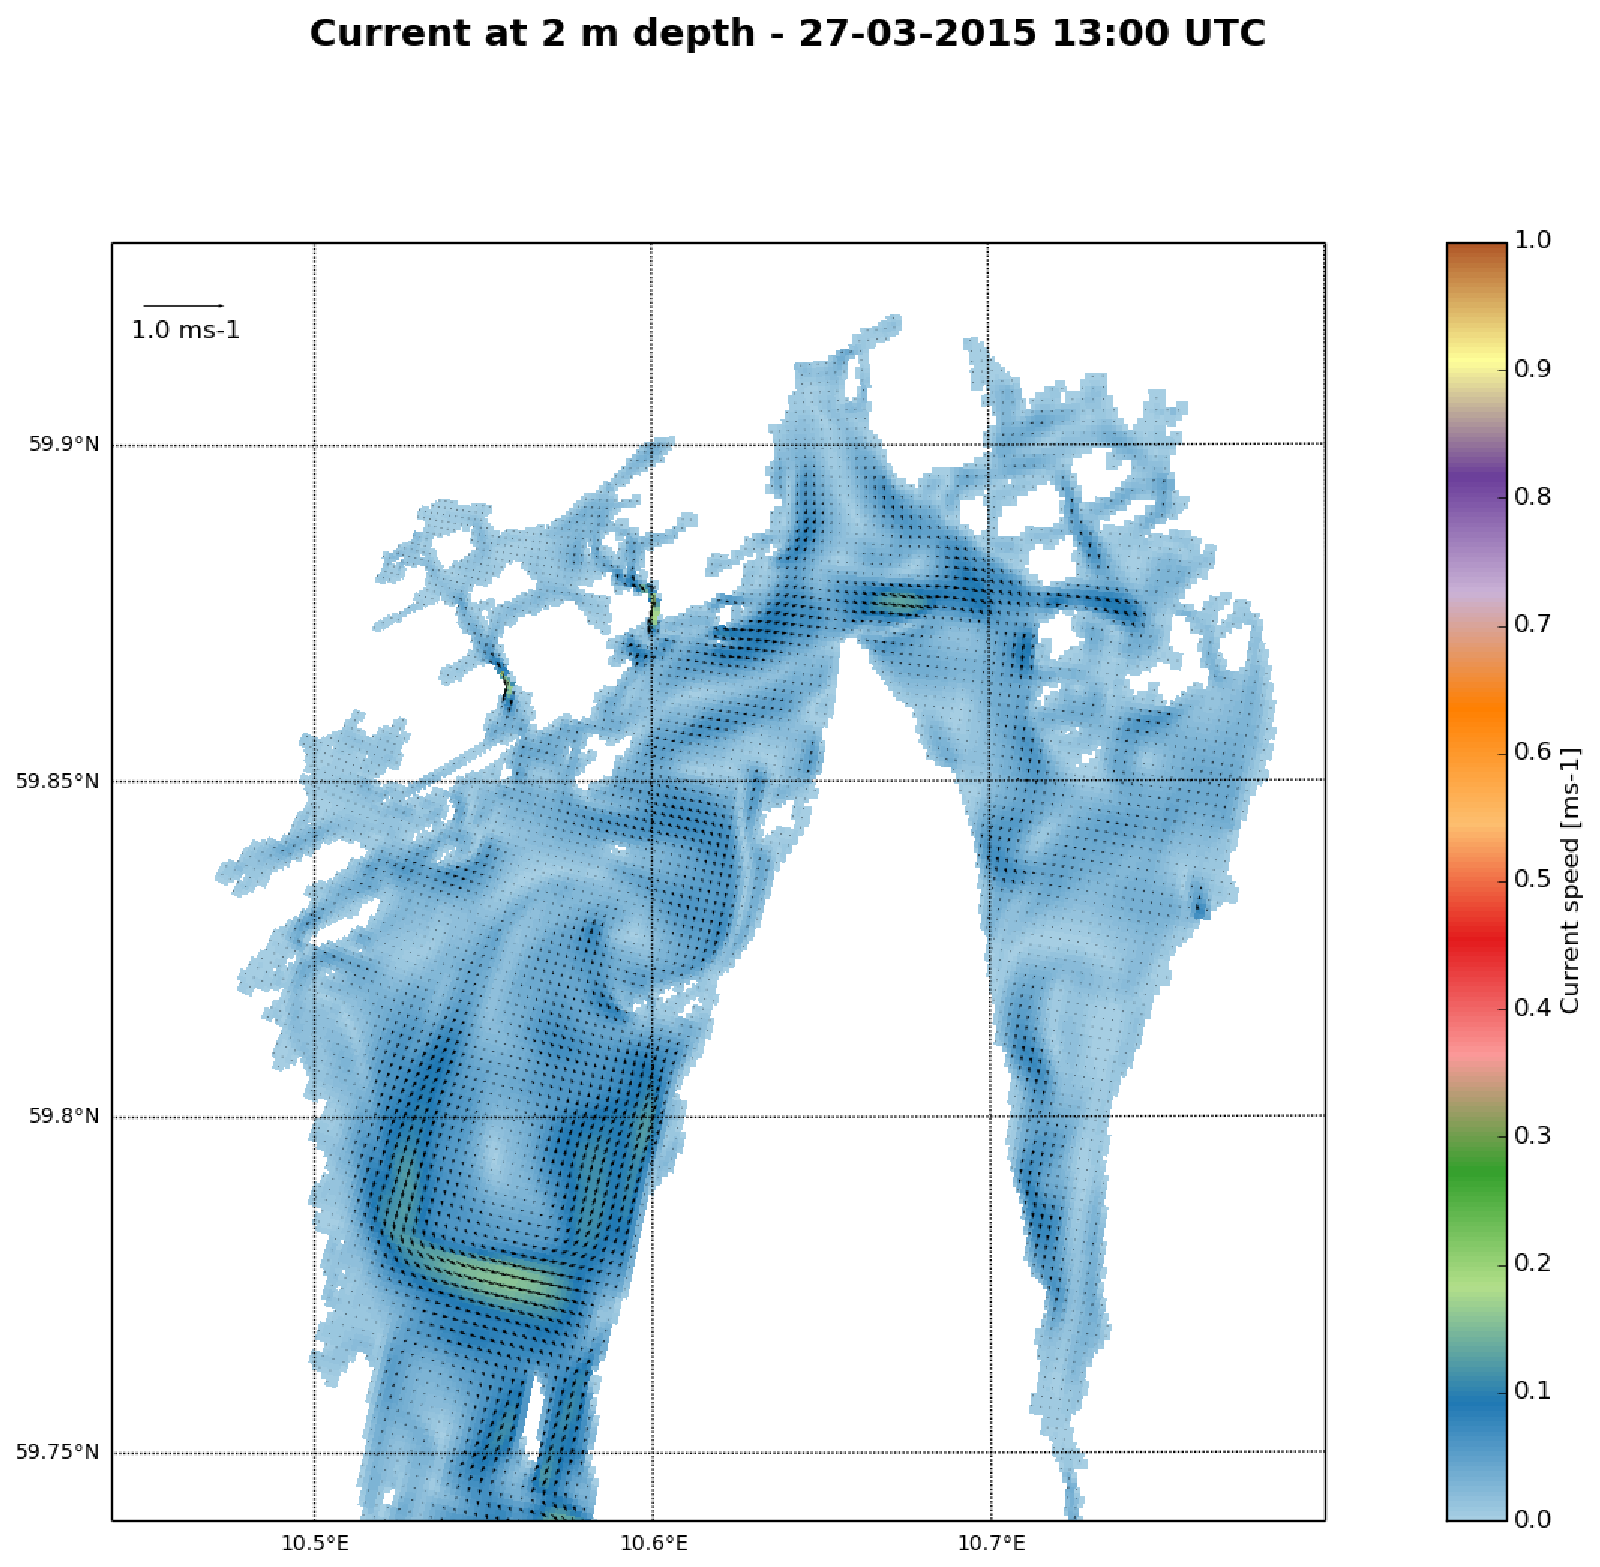
\includegraphics[height=12cm]{kap5/ferder1__0_current_crop}}
  \end{pspicture}
  \caption{\small  Currents .  }
  \label{fig:curr_oslo}
\end{figure}



As revealed by Figure \ref{fig:curr_drobak} the speed in the {\DR} Sound is much stronger with speeds bordering on 1 m/s. We also note the presence of the Jetty obstructing the western southward flow to pass through the two narrow openings in the Jetty. The picture is one of a strong outflow in which the flow in the {\DR} Sound is a jet hugging more or less the western bank due to the effect of the Earth's rotation.   
 %%%%%%%%%%%%%%%%%%% Figure  %%%%%%%%%%%%%%%
\begin{figure}[t]
  \begin{pspicture}(0,0)(15,14)
% Include graphs
	\rput[b](7.5,-0.5){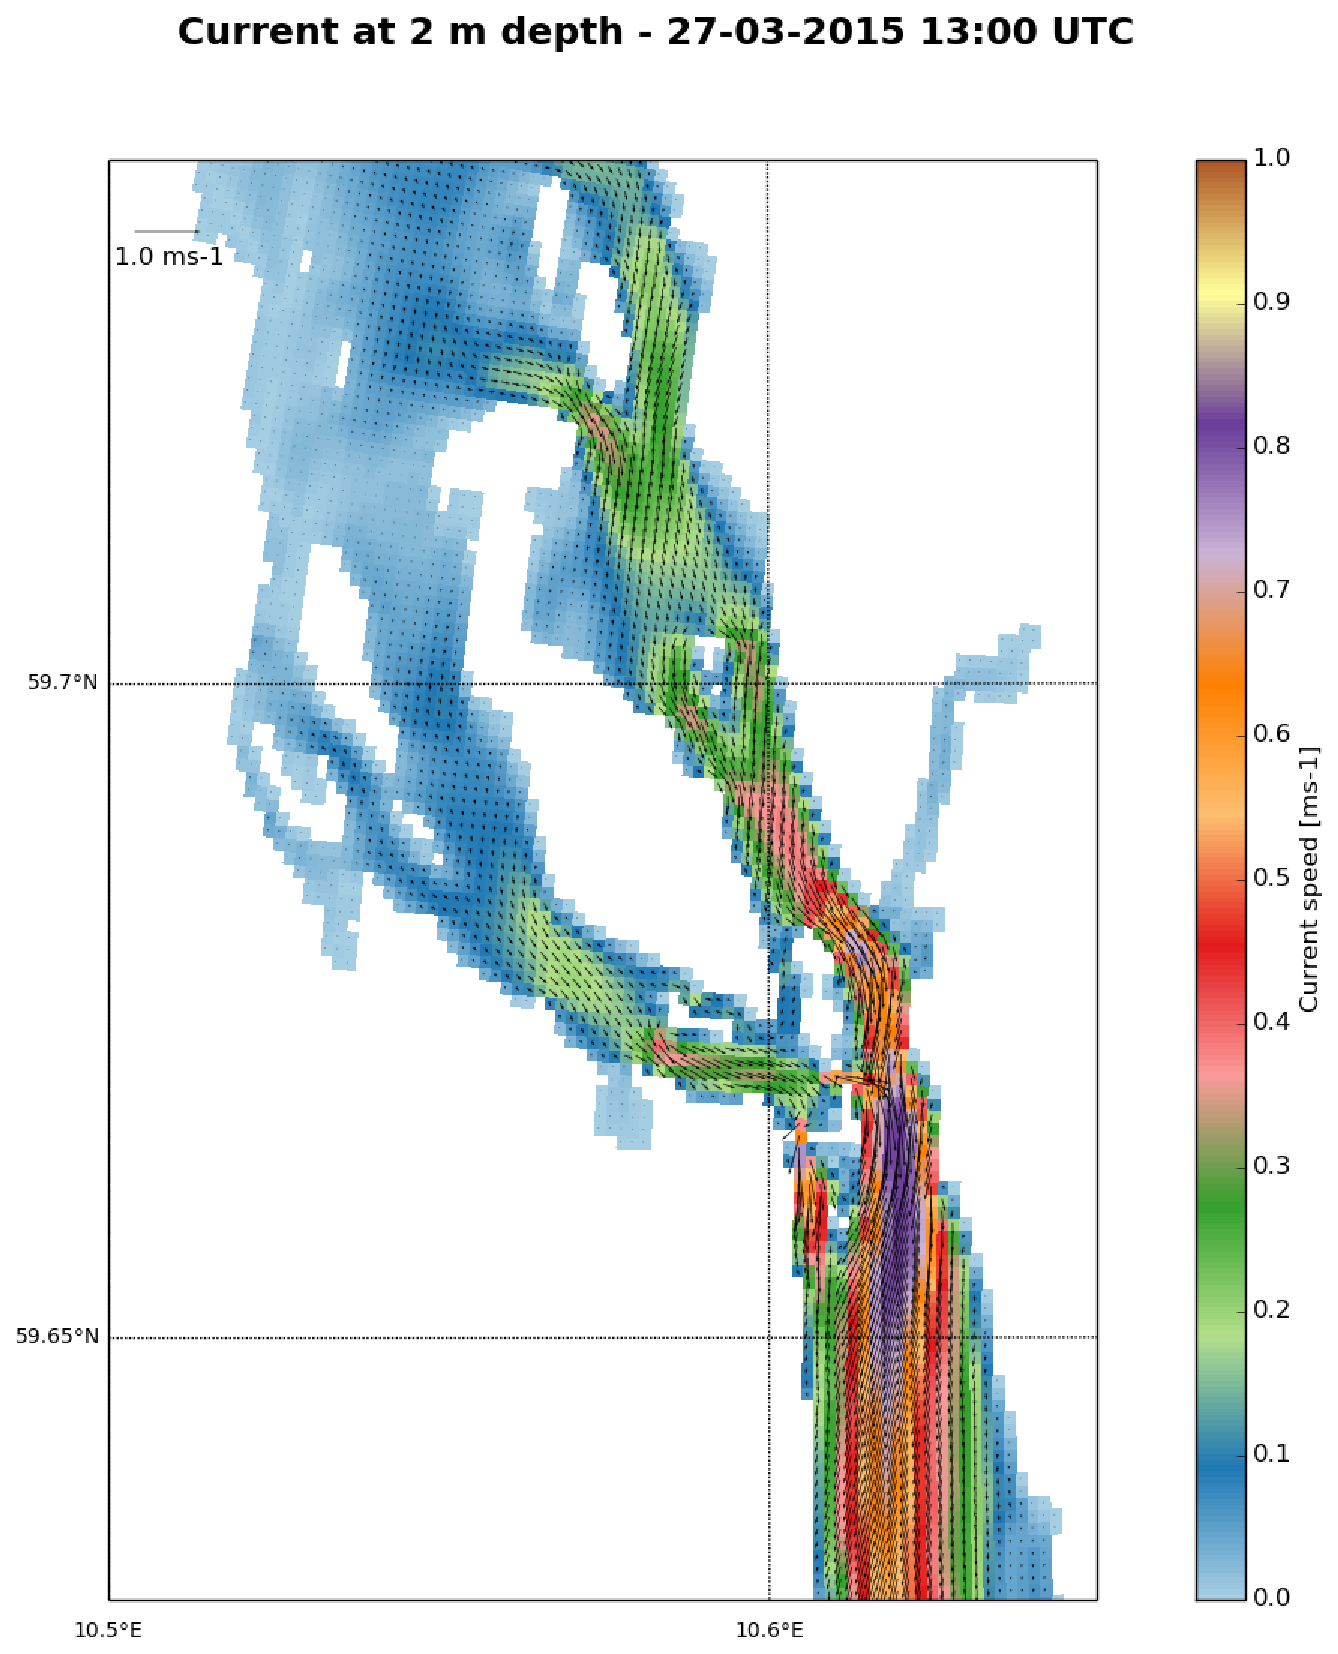
\includegraphics[height=14.5cm]{kap5/ferder2__0_current_crop}}
  \end{pspicture}
  \caption{\small As Figure \ref{fig:curr_oslo}, but for the Dr{\o}bak Sound and Vestfjorden area.}
  \label{fig:curr_drobak}
\end{figure}



As we proceed southwards into Breiangen the fjord widens. The jetlike outflow feature is clearly visible, but with rich details in the current patterns on its flanks (Figure \ref{fig:curr_breiangen}). Also Drammenselva is discharging its water into Breiangen through the Drammensfjord as revealed by Figure \ref{fig:curr_drammen}. We observe that the the simulation replicated the swift current through the narrow opening between Drammensfjorden and Breiangen at Svelvik, again forming a jetlike structure.  
\clearpage
 %%%%%%%%%%%%%%%%%%% Figure  %%%%%%%%%%%%%%%
\begin{figure}[t]
  \begin{pspicture}(0,0)(15,12)
% Include graphs
	\rput[b](7.5,0){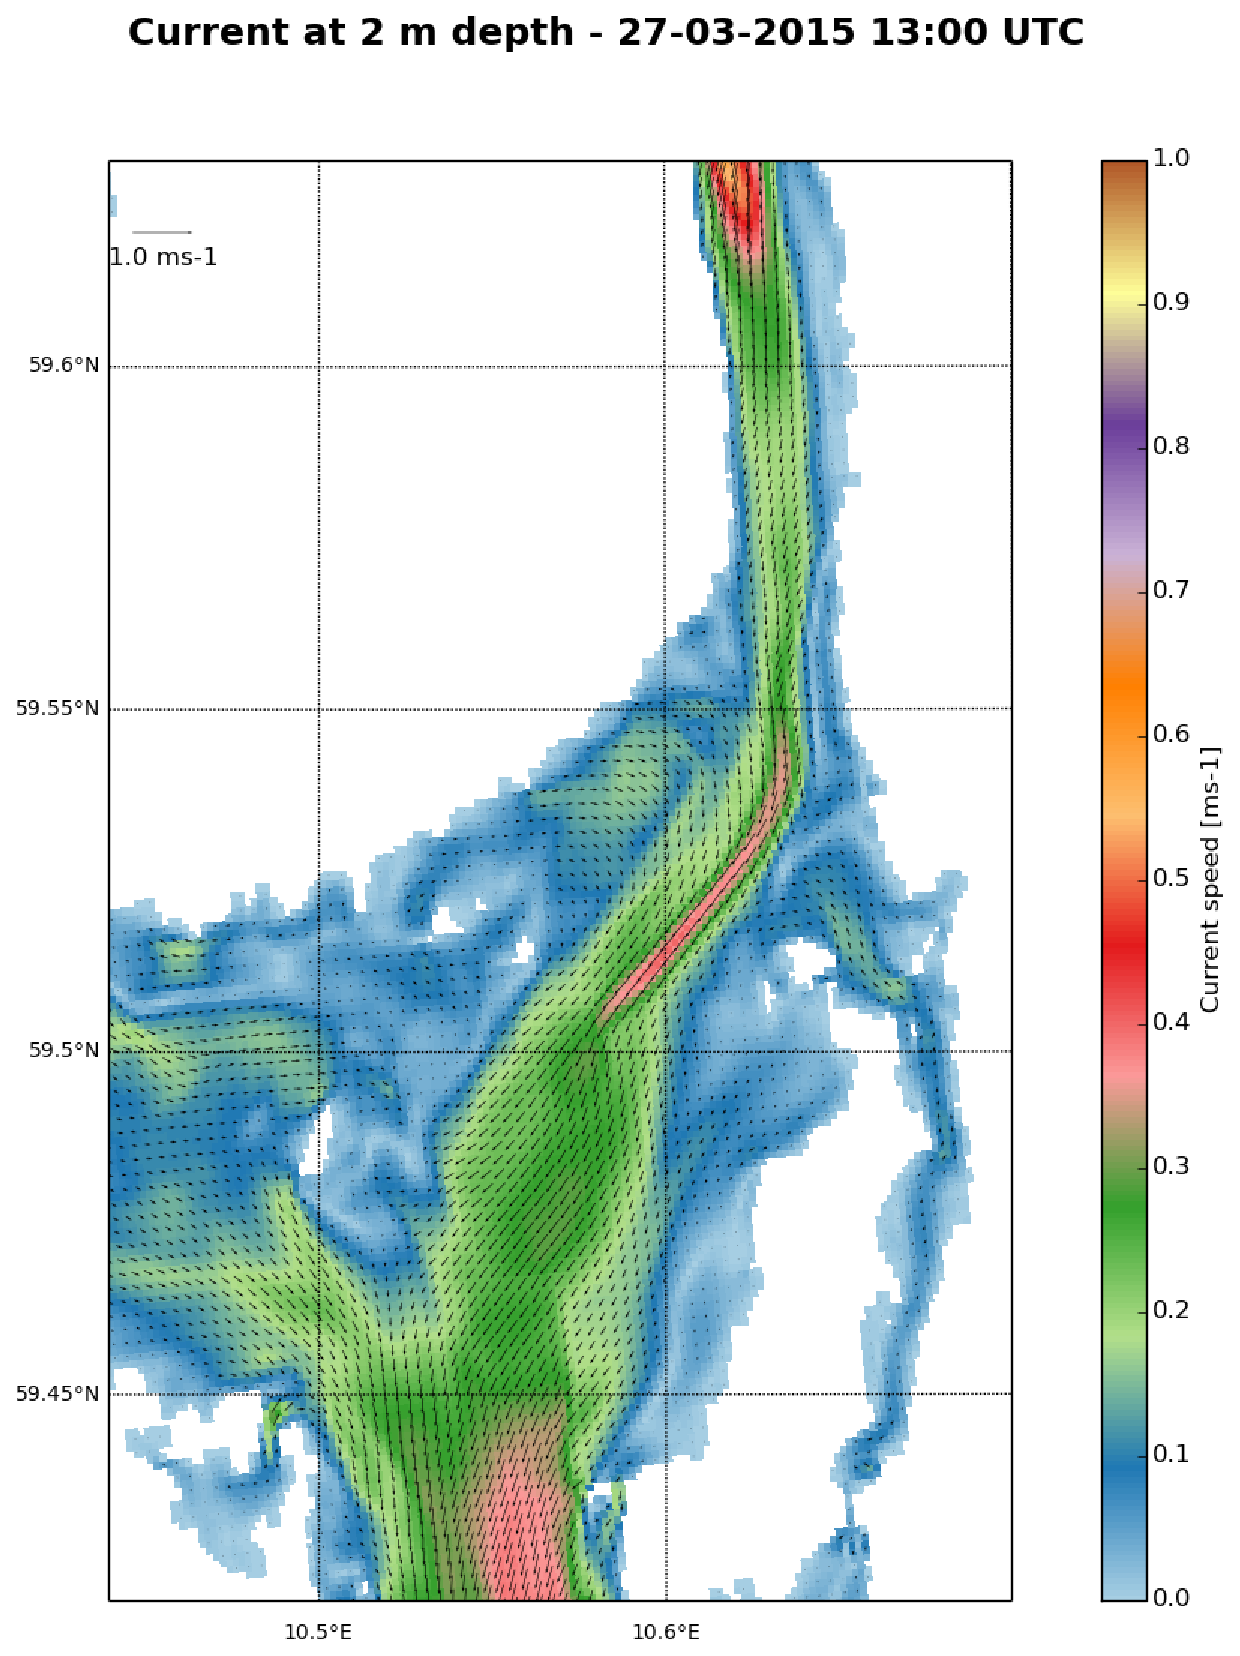
\includegraphics[height=12cm]{kap5/ferder3__0_current_crop}}
  \end{pspicture}
  \caption{\small  As for figure \ref{fig:curr_oslo}, but for the southern part of the Dr{\o}bakssund and Breidangen area.  }
  \label{fig:curr_breiangen}
\end{figure}

  
 %%%%%%%%%%%%%%%%%%% Figure  %%%%%%%%%%%%%%%
\begin{figure}[t]
  \begin{pspicture}(0,0)(15,16)
% Include graphs
	\rput[b](7.5,0){
\includegraphics[height=16cm]{kap5/drammen1__0_current_crop}}
  \end{pspicture}
  \caption{\small  As for figure \ref{fig:curr_oslo}, but for the Drammensfjord and western Breidangen area.  }
  \label{fig:curr_drammen}
\end{figure}



  
 %%%%%%%%%%%%%%%%%%% Figure  %%%%%%%%%%%%%%%
\begin{figure}[t]
  \begin{pspicture}(0,0)(15,16)
% Include graphs
	\rput[b](7.5,0){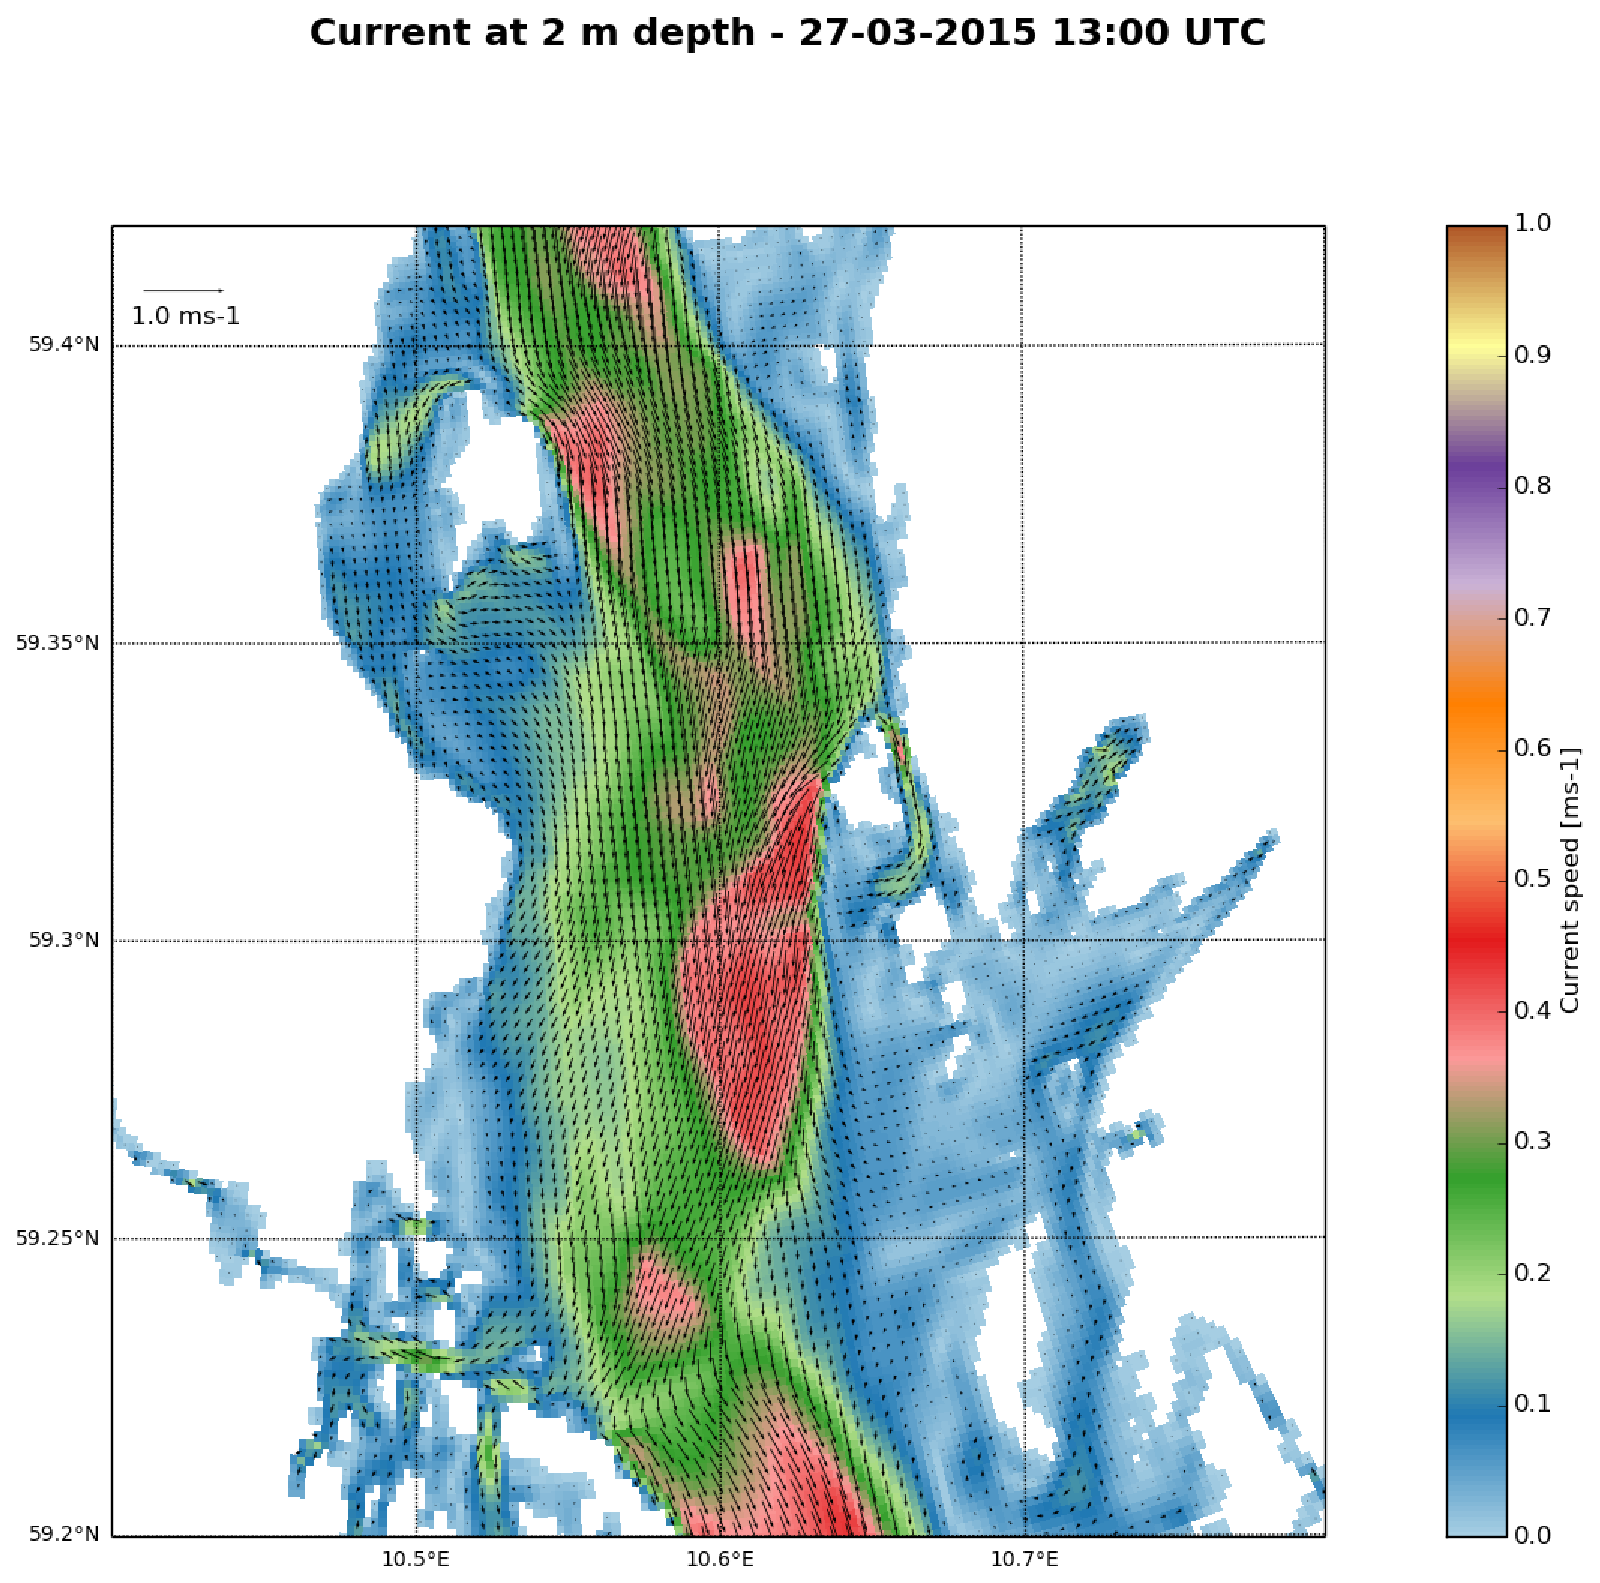
\includegraphics[height=16cm]{kap5/ferder4__0_current_crop}}
  \end{pspicture}
  \caption{\small  As Figure \ref{fig:curr_oslo}, but for the area between the Bast{\o}y, Rauer and Bol{\ae}rne islands.  }
  \label{fig:curr_mefjord}
\end{figure}

  
 %%%%%%%%%%%%%%%%%%% Figure  %%%%%%%%%%%%%%%
\begin{figure}[t]
  \begin{pspicture}(0,0)(15,12)
% Include graphs
	\rput[b](7.5,0){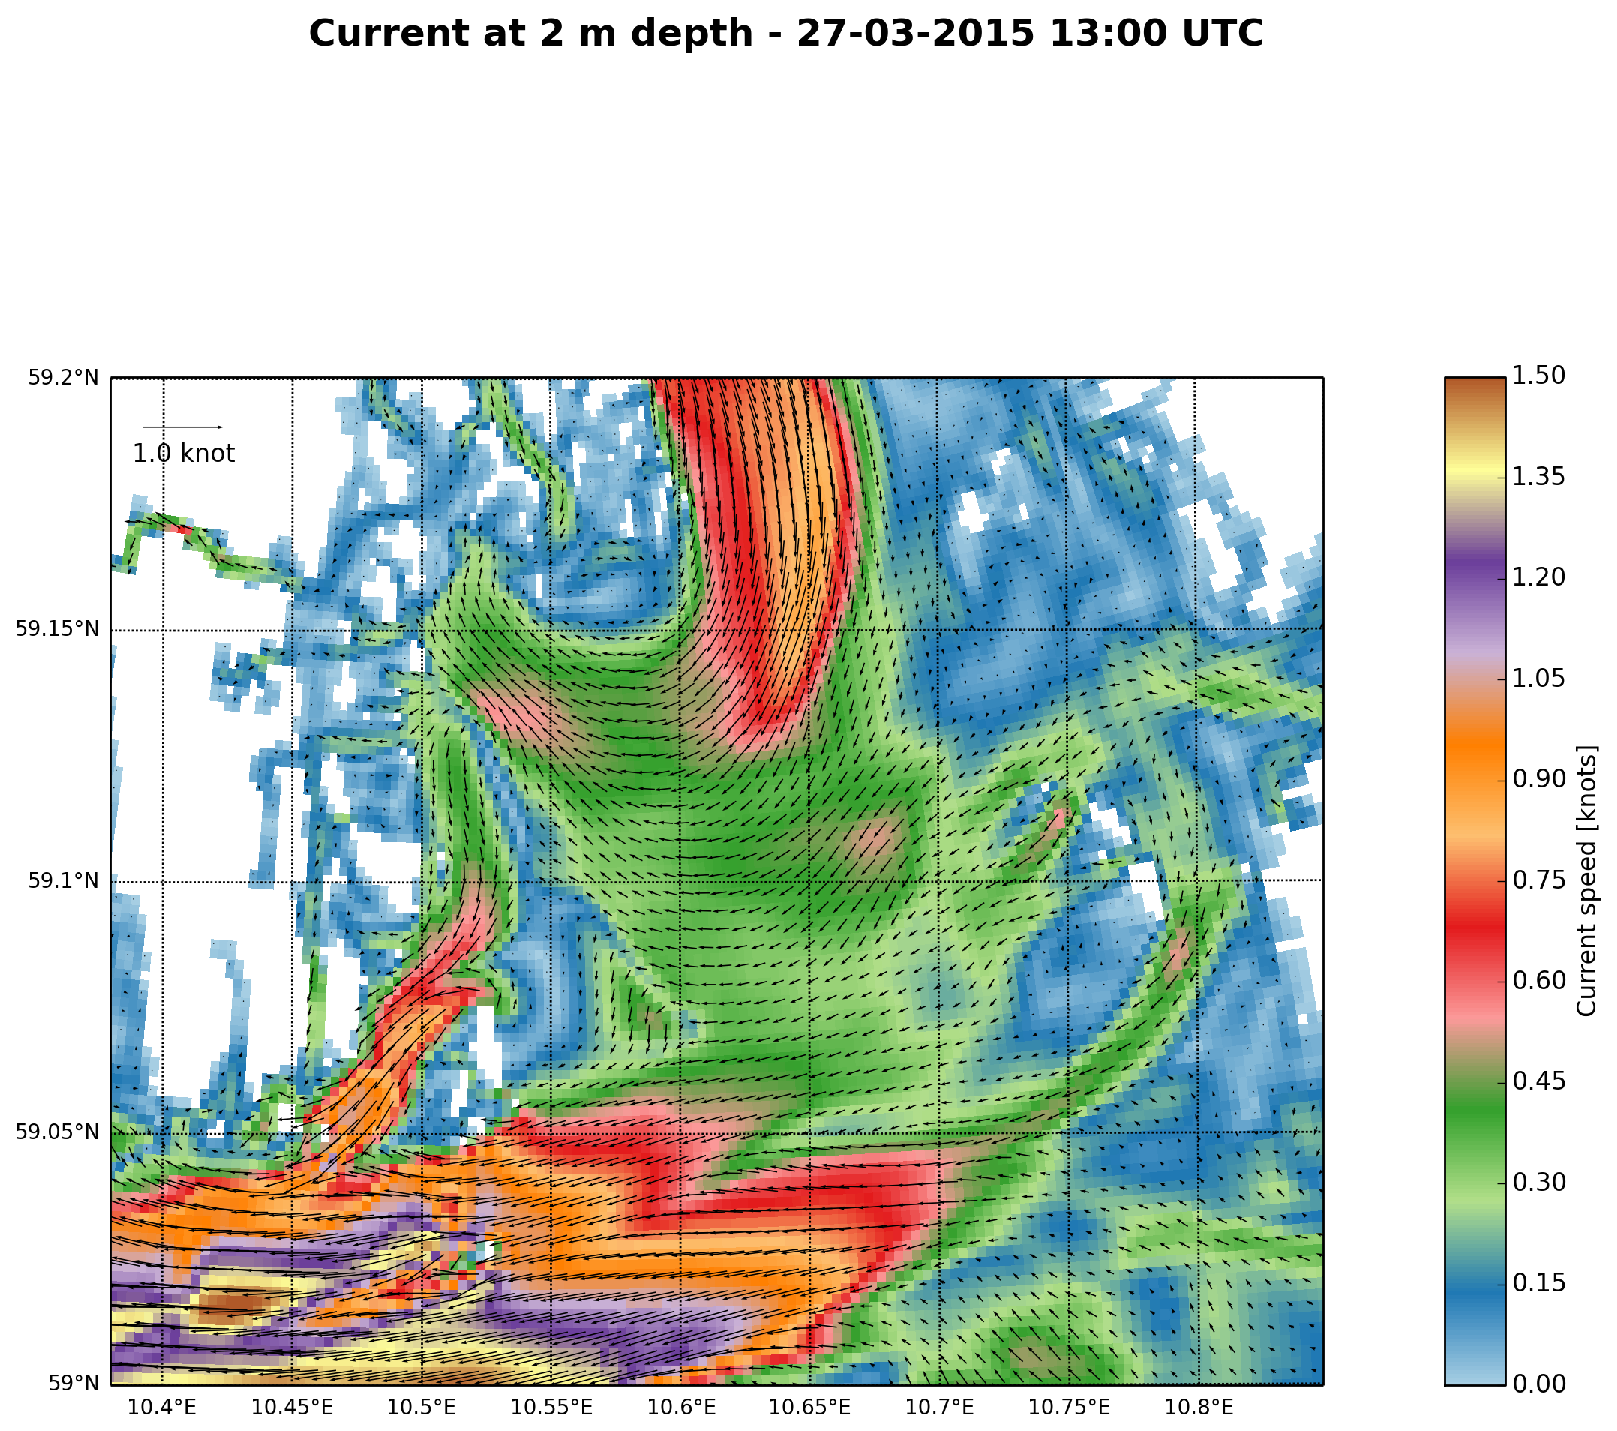
\includegraphics[height=12cm]{kap5/ferder5__0_current_crop}}
  \end{pspicture}
  \caption{\small  As for figure \ref{fig:curr_oslo}, but for the area around the F{\ae}rder lighthouse.  }
  \label{fig:curr_faerder}
\end{figure}

  

\subsection{Temperature}
\label{subsec:tempe}
 %%%%%%%%%%%%%%%%%%% Figure  %%%%%%%%%%%%%%%
\begin{figure}[t]
  \begin{pspicture}(0,0)(15,12)
% Include graphs
	\rput[b](7.5,0){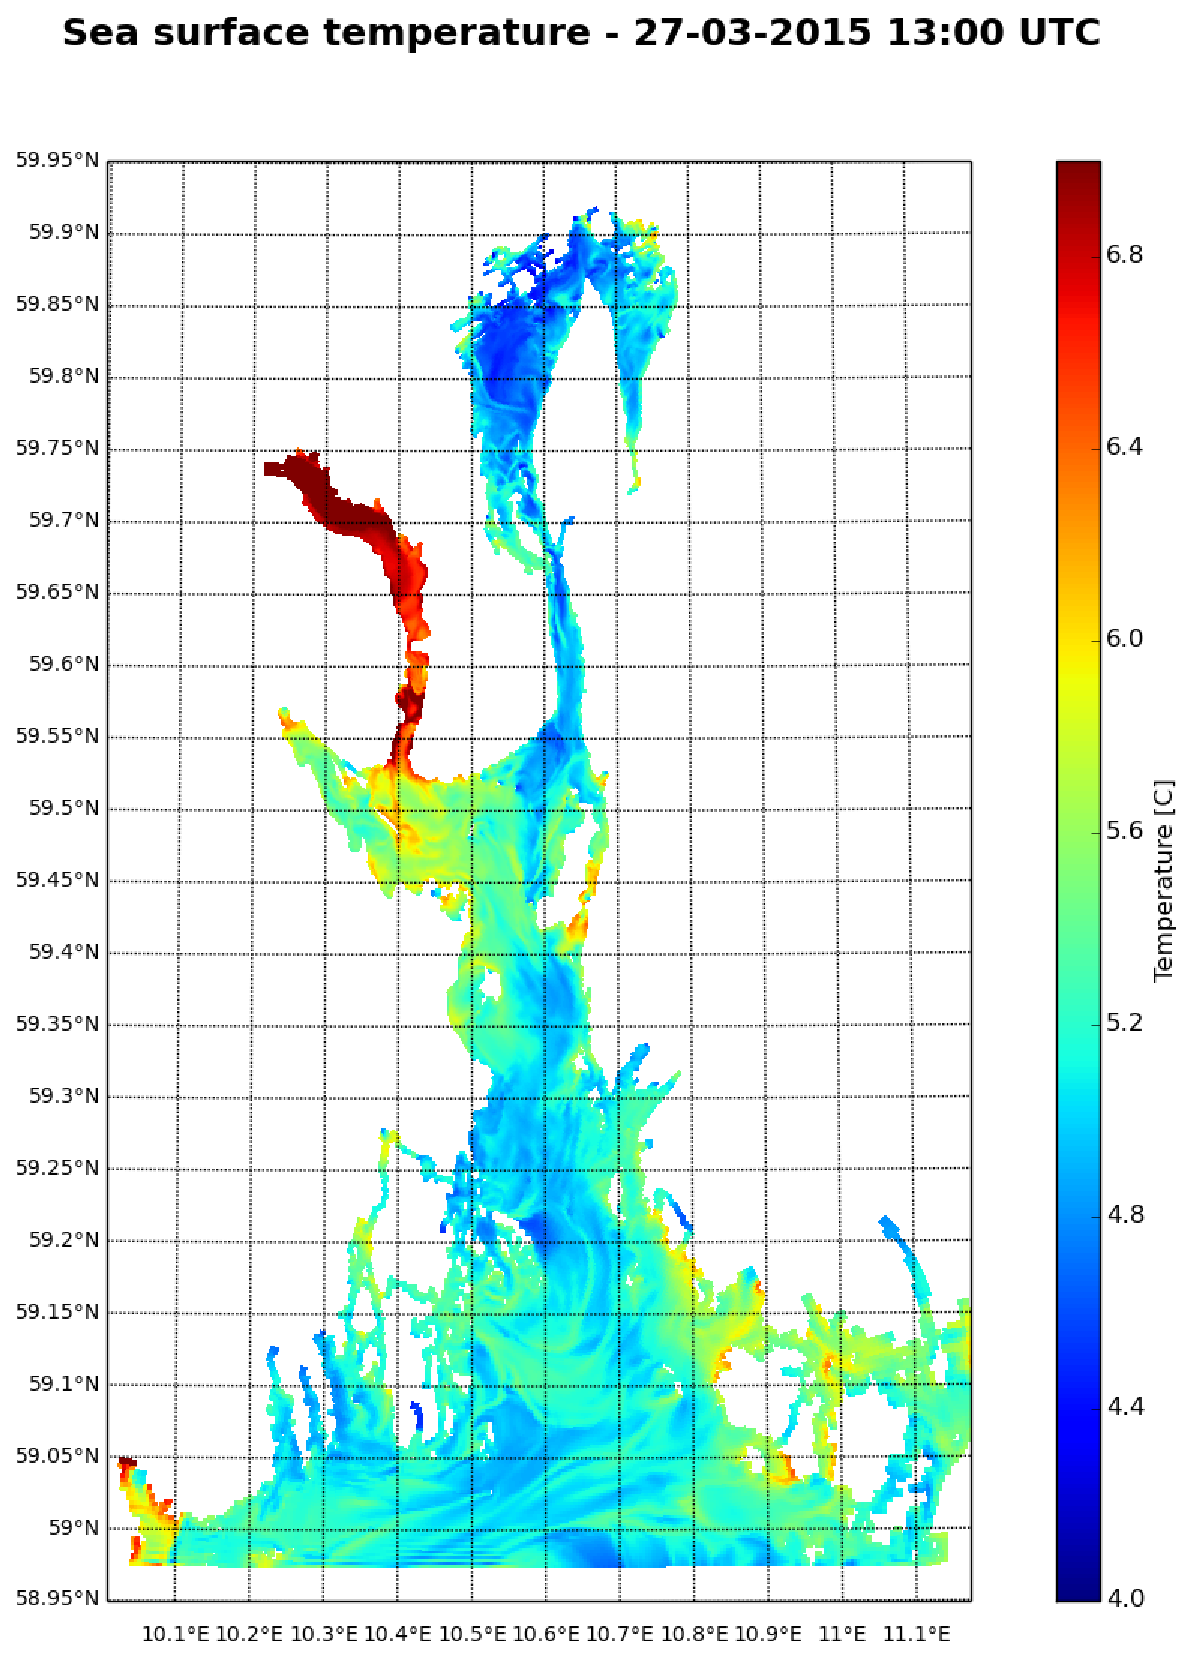
\includegraphics[height=12cm]{kap5/temp_hele_0_current_crop}}
  \end{pspicture}
  \caption{\small  Sea surface temperature (SST) for the entire model domain of the FjordOs model. Note the high SST in the Drammensfjorden area. We believe this is not realistic, and is most likely cause by the mixing up of warmer water from below. This warm water is probably left from imperfect initial conditions. }
  \label{fig:temp_hele}
\end{figure}

  

\subsection{Salinity}
\label{subsec:salin}
 %%%%%%%%%%%%%%%%%%% Figure  %%%%%%%%%%%%%%%
\begin{figure}[t]
  \begin{pspicture}(0,0)(15,12)
% Include graphs
	\rput[b](7.5,0){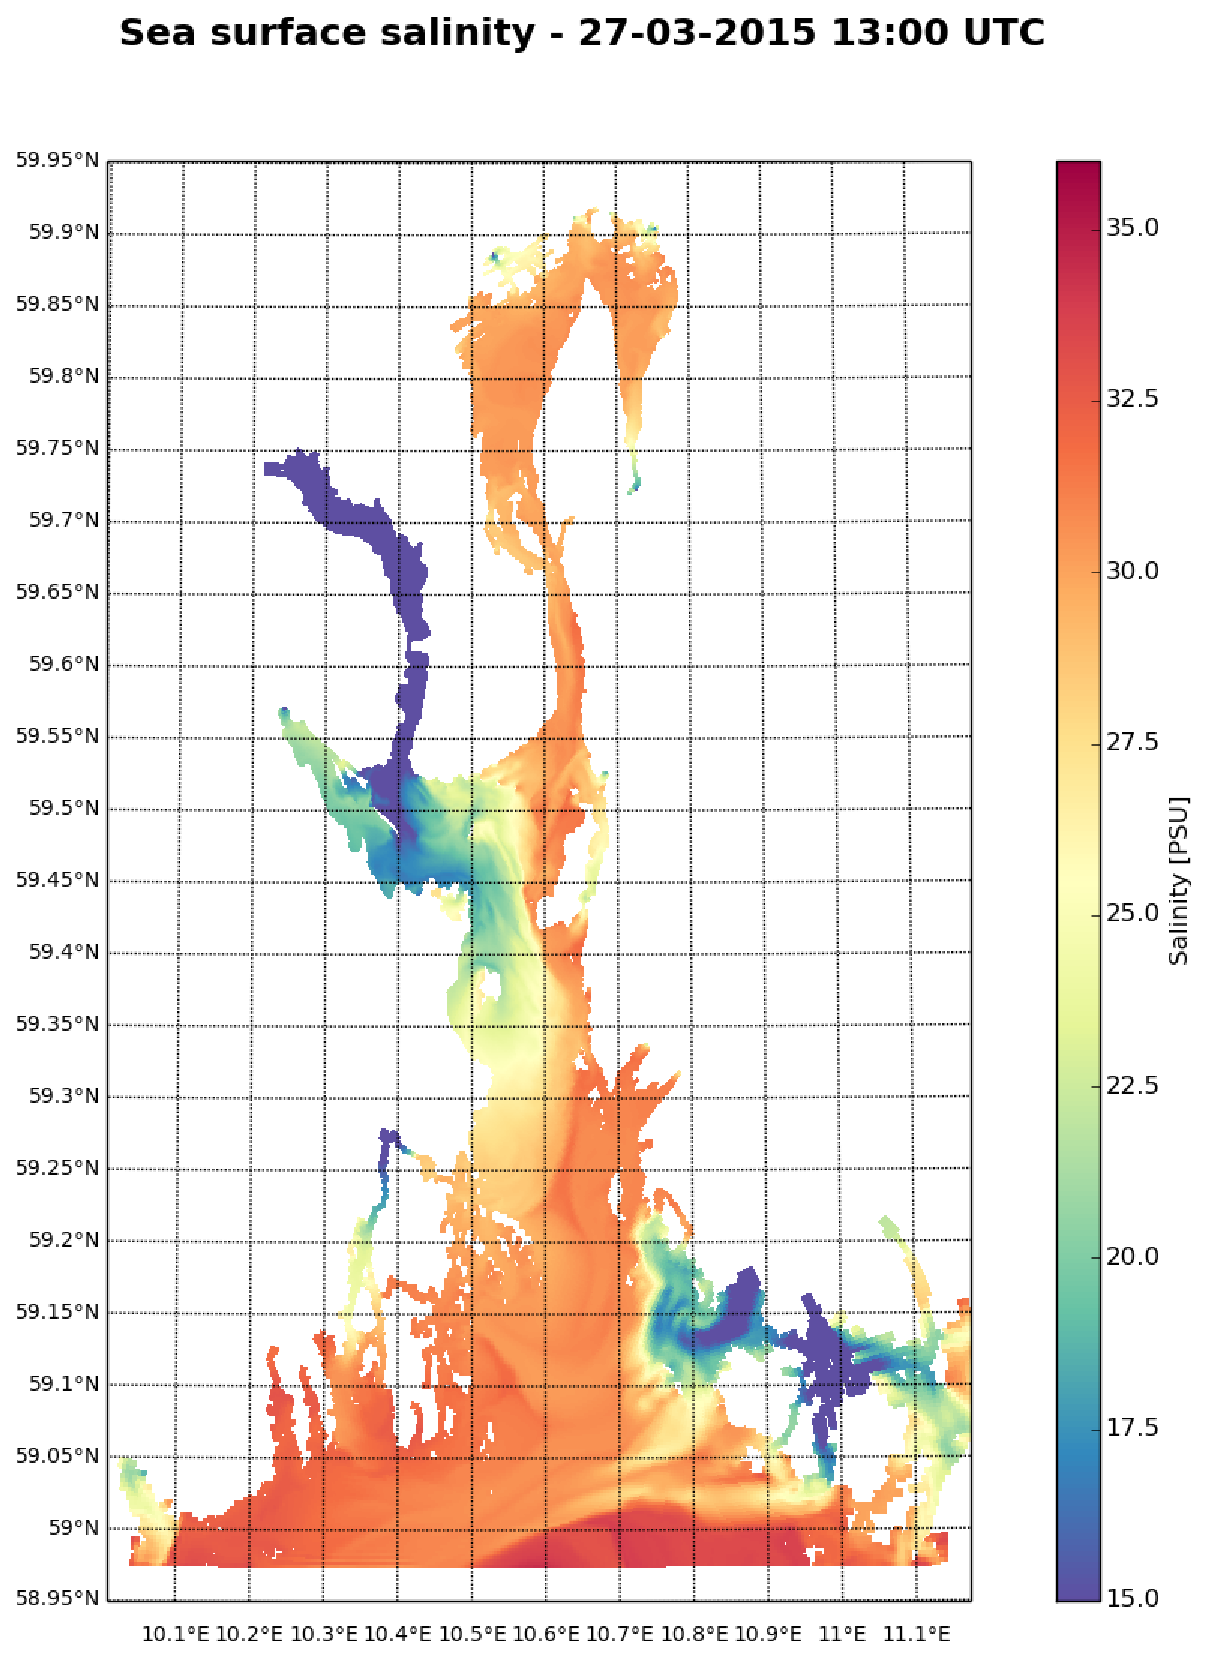
\includegraphics[height=12cm]{kap5/salt_hele_0_current_crop}}
  \end{pspicture}
  \caption{\small  As for figure \ref{fig:temp_hele}, but for sea surface salinity (SSS).  }
  \label{fig:salt_hele}
\end{figure}

  

\subsubsection{Sea level}
\label{subsec:seale}
 %%%%%%%%%%%%%%%%%%% Figure  %%%%%%%%%%%%%%%
\begin{figure}[t]
  \begin{pspicture}(0,0)(15,17)
% Include graphs
	\rput[b](7.5,0){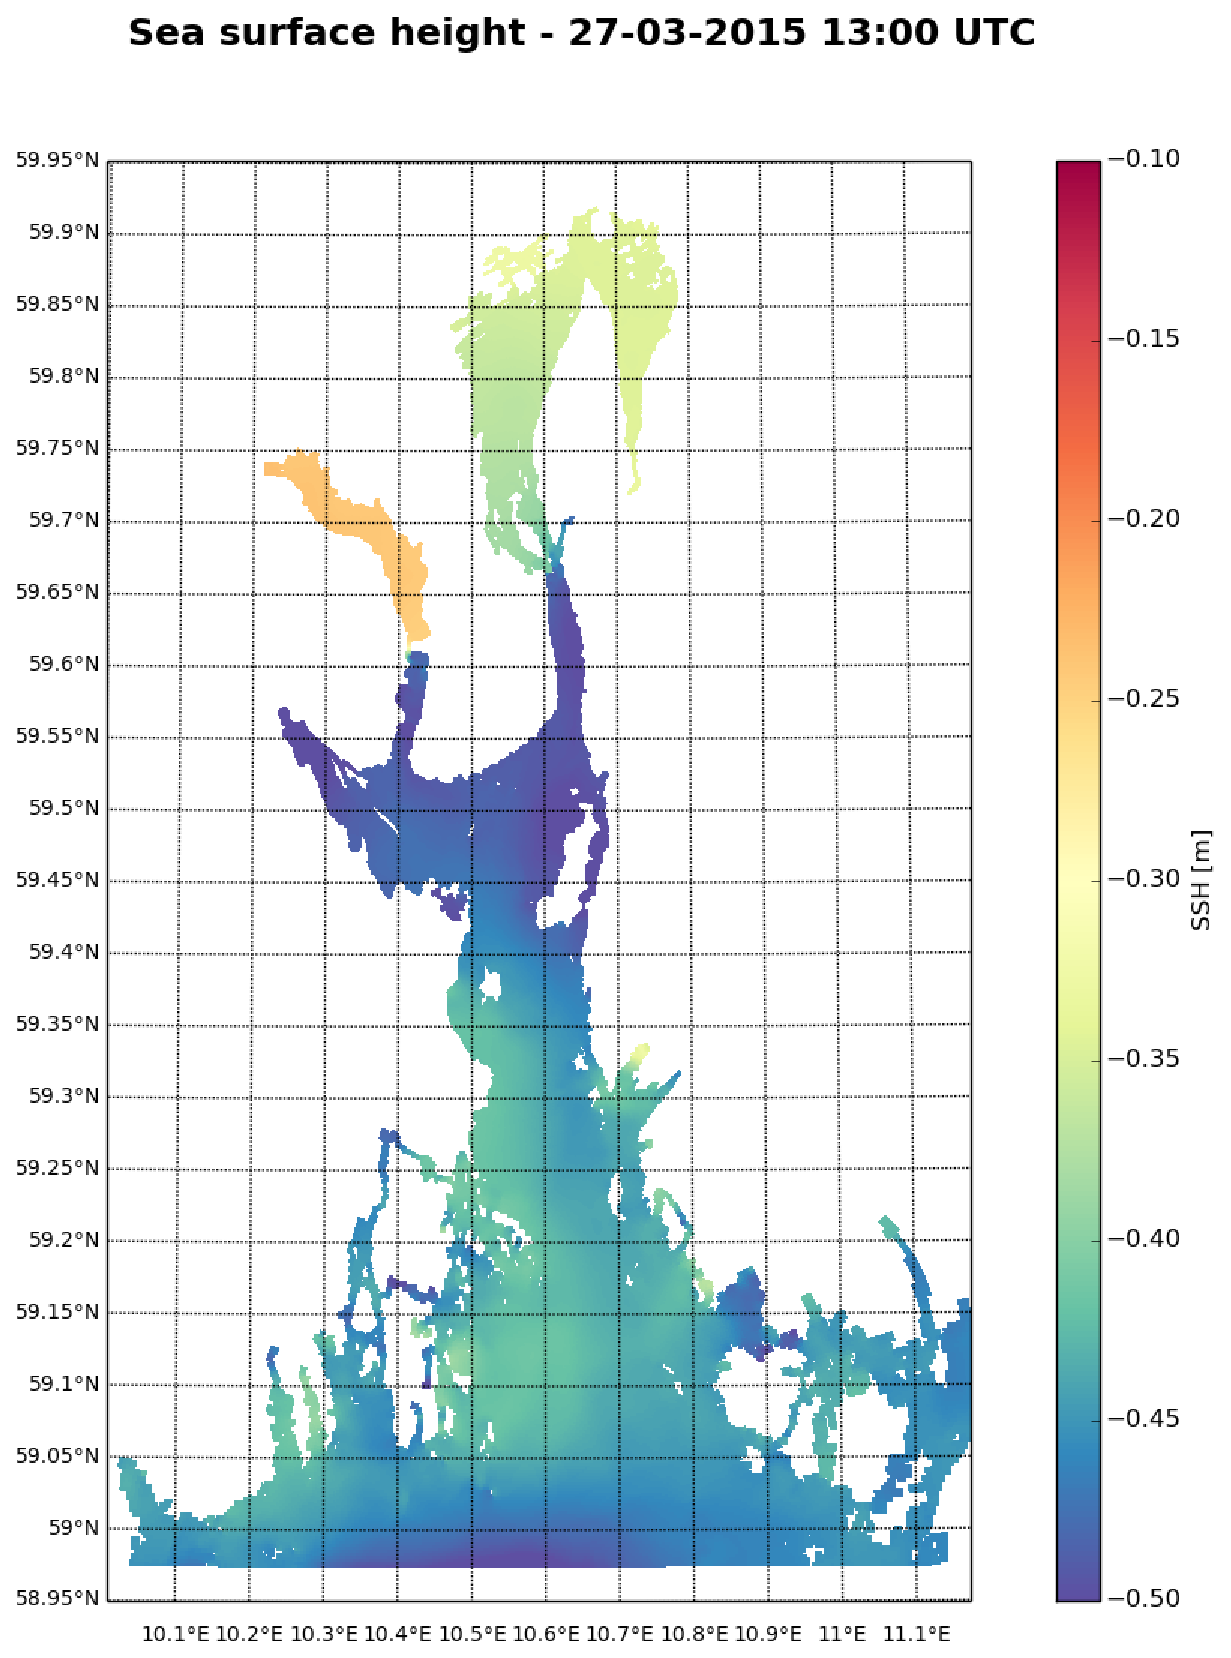
\includegraphics[height=17cm]{kap5/zeta_hele_0_crop}}
  \end{pspicture}
  \caption{\small  As for figure \ref{fig:temp_hele}, but for sea surface height (SSH).  }
  \label{fig:ssh_hele}
\end{figure}

  
\clearpage
